%----------------------------------------------------------------------------
\chapter{Jegyzőkönyv}
%----------------------------------------------------------------------------

%----------------------------------------------------------------------------
\section{Első feladat}
%----------------------------------------------------------------------------
Direkt első típusú vagy indirekt második típusú Sugeno-fuzzy irányítást kellett megvalósítanunk a mérés során. A mérőcsoportunk a direkt első típusú irányítást választotta. A direkt irányítás lényege, hogy közvetlenül a beavatkozó jelre adunk egy becslést. Első típusú, mivel csak a szabályok kimenetét hangoljuk. Ehhez a segédlet (28)-as képleteit kellett felhasználnunk:

\begin{figure}[!h]
	\centering
	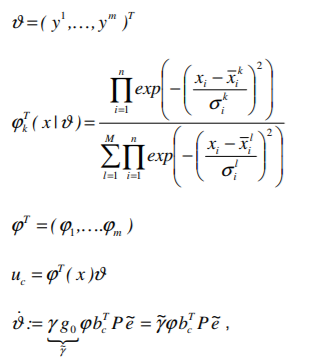
\includegraphics[width=91mm, keepaspectratio]{figures/m03/fig1.png}
	\label{fig:fig1}
\end{figure}


A kapott keretprogram tartalmazta a megfelelő képletek implementációját.
A kód vizsgálata és megértése után a hiányzó részek kitöltése következett.



\newpage
%----------------------------------------------------------------------------
\section{Második feladat}
%----------------------------------------------------------------------------
Elsőként a Lambdát és P-t kellett meghatároznunk. Lambda a segédlet 9-es pontjában található képlet segítségével számolható.

\begin{figure}[!h]
	\centering
	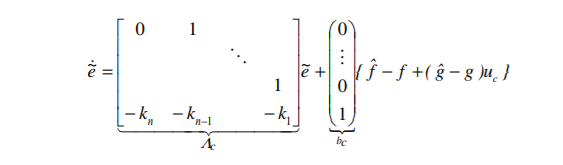
\includegraphics[width=91mm, keepaspectratio]{figures/m03/fig2.png}
	\label{fig:fig1}
\end{figure}


P kiszámítása a következő összefüggésből adódott:

\begin{figure}[!h]
	\centering
	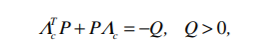
\includegraphics[width=61mm, keepaspectratio]{figures/m03/fig3.png}
	\label{fig:fig1}
\end{figure}
A P és Lambda kész kódja:

\begin{figure}[!h]
	\centering
	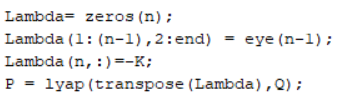
\includegraphics[width=91mm, keepaspectratio]{figures/m03/fig4.png}
	\label{fig:fig1}
\end{figure}
Az Uc, Us, U meghatározása:

\begin{figure}[!h]
	\centering
	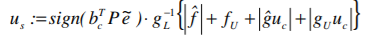
\includegraphics[height=10mm, keepaspectratio]{figures/m03/fig5.png}\\\vspace{5mm}\hspace{5mm}
	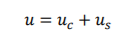
\includegraphics[height=12mm, keepaspectratio]{figures/m03/fig6.png}\vspace{5mm}
	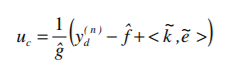
\includegraphics[height=14mm, keepaspectratio]{figures/m03/fig7.png}
	\label{fig:Dejong}
\end{figure}

\begin{figure}[!h]
\centering
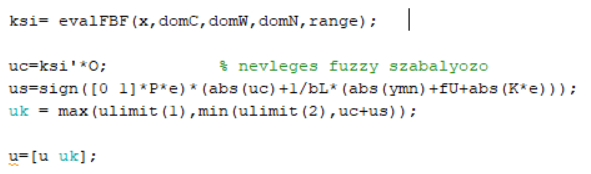
\includegraphics[width=111mm, keepaspectratio]{figures/m03/fig8.png}
\label{fig:fig1}
\end{figure}
\newpage

Látható, hogy a szabályzó szépen követi a referencia szinusz jelet. A „rezgések” a felügyelő szabályzó használata miatt jelennek meg.

\begin{figure}[!h]
	\centering
	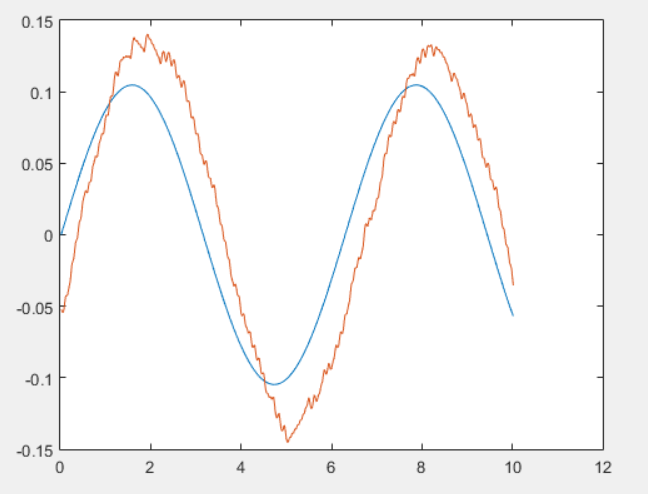
\includegraphics[width=111mm, keepaspectratio]{figures/m03/fig9.png}
	\label{fig:fig1}
\end{figure}






